% ----------------------------------------------------------
% Desenvolvimento
% ----------------------------------------------------------
\chapter{Desenvolvimento}

\section{Fundamentação Teórica e Trabalhos Relacionados}

Para o projeto de robôs seguidores de linha, a locomoção com acionamento diferencial é a mais empregada por sua simplicidade e precisão mecânica. Essa configuração utiliza duas rodas motrizes independentes e uma roda de apoio (caster). O modelo cinemático baseia-se nas velocidades lineares das rodas esquerda ($v_L$) e direita ($v_R$) para determinar a velocidade linear global ($v$) e a velocidade angular ($\omega$) do centro de massa do robô \cite{siegwart2011introduction}. A correta tradução desses modelos matemáticos para a execução física é um desafio clássico em sistemas de tempo real, onde a latência de processamento e o atrito do solo introduzem variações não modeladas \cite{vega2025bridging}.

\subsection{Controle PID (Proporcional-Integral-Derivativo)}

Para o controle preciso da trajetória, implementou-se o algoritmo PID (Proporcional-Integral-Derivativo). Embora a teoria clássica baseie-se no tempo contínuo, a execução no Raspberry Pi 4 exige uma aproximação discreta, conforme apresentada na Equação \ref{eq:pid_discreto}. Esta formulação permite que o controlador processe o erro de posição em intervalos de tempo fixos ($\Delta t$), garantindo a estabilidade dinâmica do sistema \cite{ferreira2023differential, baluja2024design, stark2026development}:

\begin{equation}
    u(k) = K_p e(k) + K_i \sum_{i=0}^{k} e(i) \Delta t + K_d \frac{e(k) - e(k-1)}{\Delta t}
    \label{eq:pid_discreto}
\end{equation}

Os ganhos $K_p$, $K_i$ e $K_d$ foram sintonizados para responder rapidamente a desvios na linha, minimizando oscilações e compensando o erro de regime permanente.


\subsection{Middleware ROS 2 Humble e Edge Computing}

O \textit{Robot Operating System 2} (ROS 2) consolida-se por sua arquitetura distribuída baseada no padrão DDS (\textit{Data Distribution Service}), que permite comunicação sem um nó mestre centralizado. A versão Humble Hawksbill, lançada em 2022, traz melhorias significativas na eficiência de rede e suporte a sistemas embarcados modernos. 
A utilização do Raspberry Pi 4 Model B com Ubuntu 22.04 permite a aplicação de \textit{Edge Computing} (Computação de Borda). Neste paradigma, o processamento das leituras do módulo BFD-1000 e a execução da malha PID ocorrem localmente, reduzindo a latência e a dependência de conectividade externa para decisões críticas de navegação \cite{macenski2022robot, zhang2022distributed}.

\section{Metodologia e Arquitetura}

A metodologia deste trabalho é dividida entre a validação em ambiente simulado e a implementação no protótipo físico, garantindo que a lógica de controle seja testada antes do embarque no hardware real.

\begin{figure}[H]
	\caption{\label{fig:diagrama_sistema}Diagrama de blocos da arquitetura do sistema.}
	\begin{center}
	    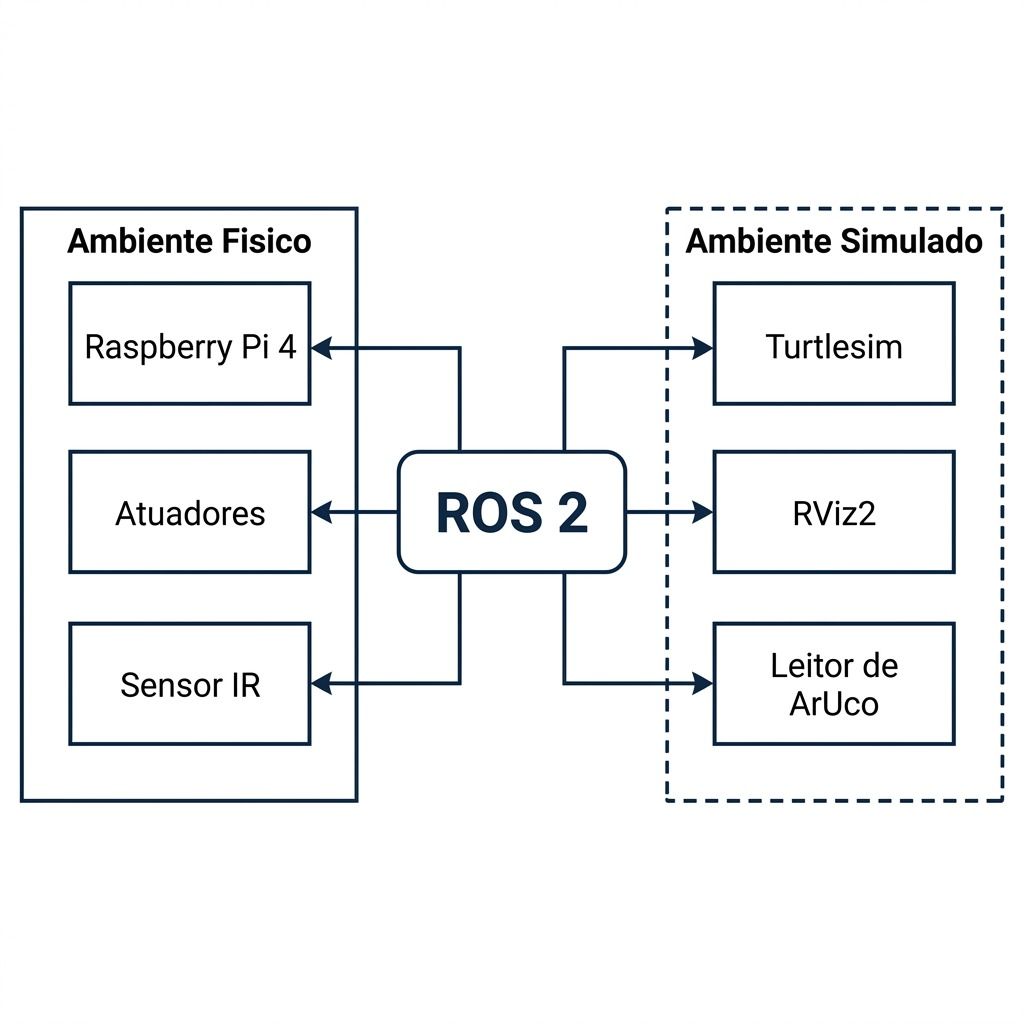
\includegraphics[width=0.6\textwidth]{imagens/arquitetura_sistema}
	\end{center}
	\legend{Fonte: Elaborado pelo autor.}
\end{figure}

A estrutura de funcionamento do projeto, abrangendo desde a inicialização dos nós no ROS 2 até o processamento sensorial e a tomada de decisão, é detalhada no fluxograma da Figura \ref{fig:fluxograma}. Este fluxo ilustra como a lógica de controle PID interage com os dados de entrada para orquestrar a movimentação física do robô.

\begin{figure}[H]
	\caption{\label{fig:fluxograma}Fluxograma de funcionamento da solução.}
	\begin{center}
	    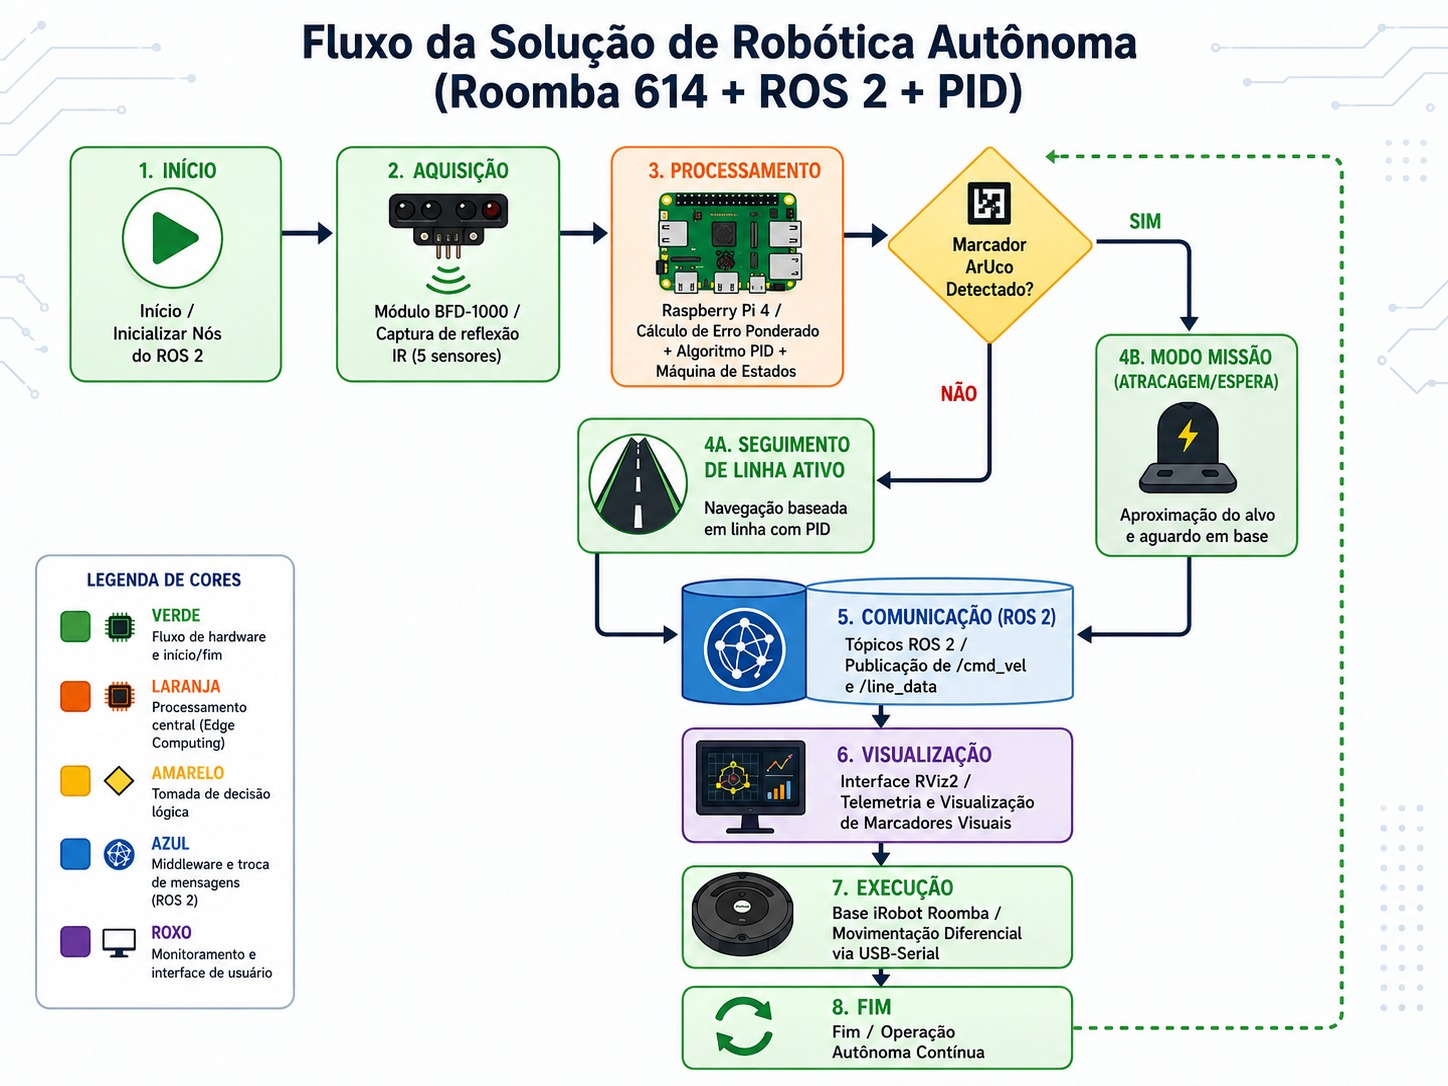
\includegraphics[width=0.75\textwidth]{imagens/fluxograma_roomba_seguidor_linha}
	\end{center}
	\legend{Fonte: Elaborado pelo autor.}
\end{figure}


\subsection{Ambiente de Simulação e Visão Computacional}

A simulação foi realizada no ambiente \textit{Turtlesim}, permitindo testar cenários de lógica de controle e navegação sem riscos ao hardware, seguindo práticas recomendadas para o ensino de robótica em sistemas baseados no ROS 2 \cite{university2024labbook}.
\begin{itemize}
    \item \textbf{Seguimento de Linha:} O robô simulado no Turtlesim utiliza vetores de movimento para validar a lógica do PID antes da tradução para o hardware real;
    \item \textbf{Visualização e ArUco no RViz2:} Implementou-se um sistema de visualização no \textit{RViz2} para localizar e identificar marcadores ArUco de forma virtual. Na simulação, esses marcadores são usados para definir "missões", como paradas obrigatórias ou mudanças de comportamento. O algoritmo utiliza a biblioteca OpenCV para o processamento de imagem em tempo real, baseando-se em modelos de estimativa de pose validados na literatura \cite{kalaitzakis2021fiducial, stangl2023analytical}. A integração desses marcadores em ambiente virtual permitiu validar, para uso futuro no hardware físico, a transição autônoma do robô entre o modo de "seguimento de linha" e o modo de "atracagem" ou "espera", com o \textit{feedback} visual centralizado no RViz2.
\end{itemize}

\begin{figure}[H]
	\caption{\label{fig:simulacao}Interface do Turtlesim integrado ao RViz2 com marcadores ArUco.}
	\begin{center}
	    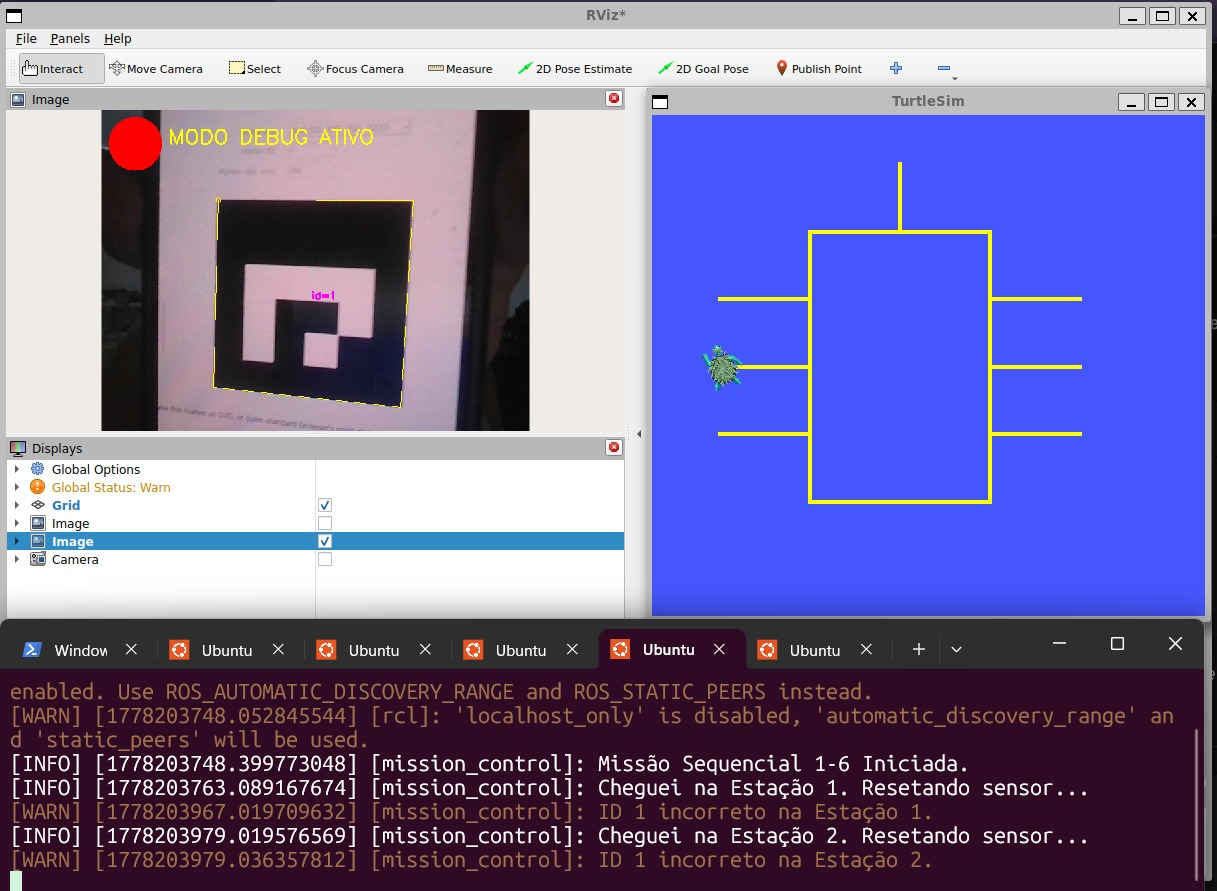
\includegraphics[width=0.6\textwidth]{imagens/simulacao_aruco}
	\end{center}
	\legend{Fonte: Elaborado pelo autor.}
\end{figure}

\subsection{Implementação Física e Hardware}

A implementação física baseia-se no iRobot Roomba (Série 600). A integração do hardware seguiu especificações rigorosas para garantir estabilidade elétrica e de sinal.

\begin{figure}[H]
	\caption{\label{fig:componentes}Principais componentes: Raspberry Pi 4 e Módulo BFD-1000.}
	\begin{center}
	    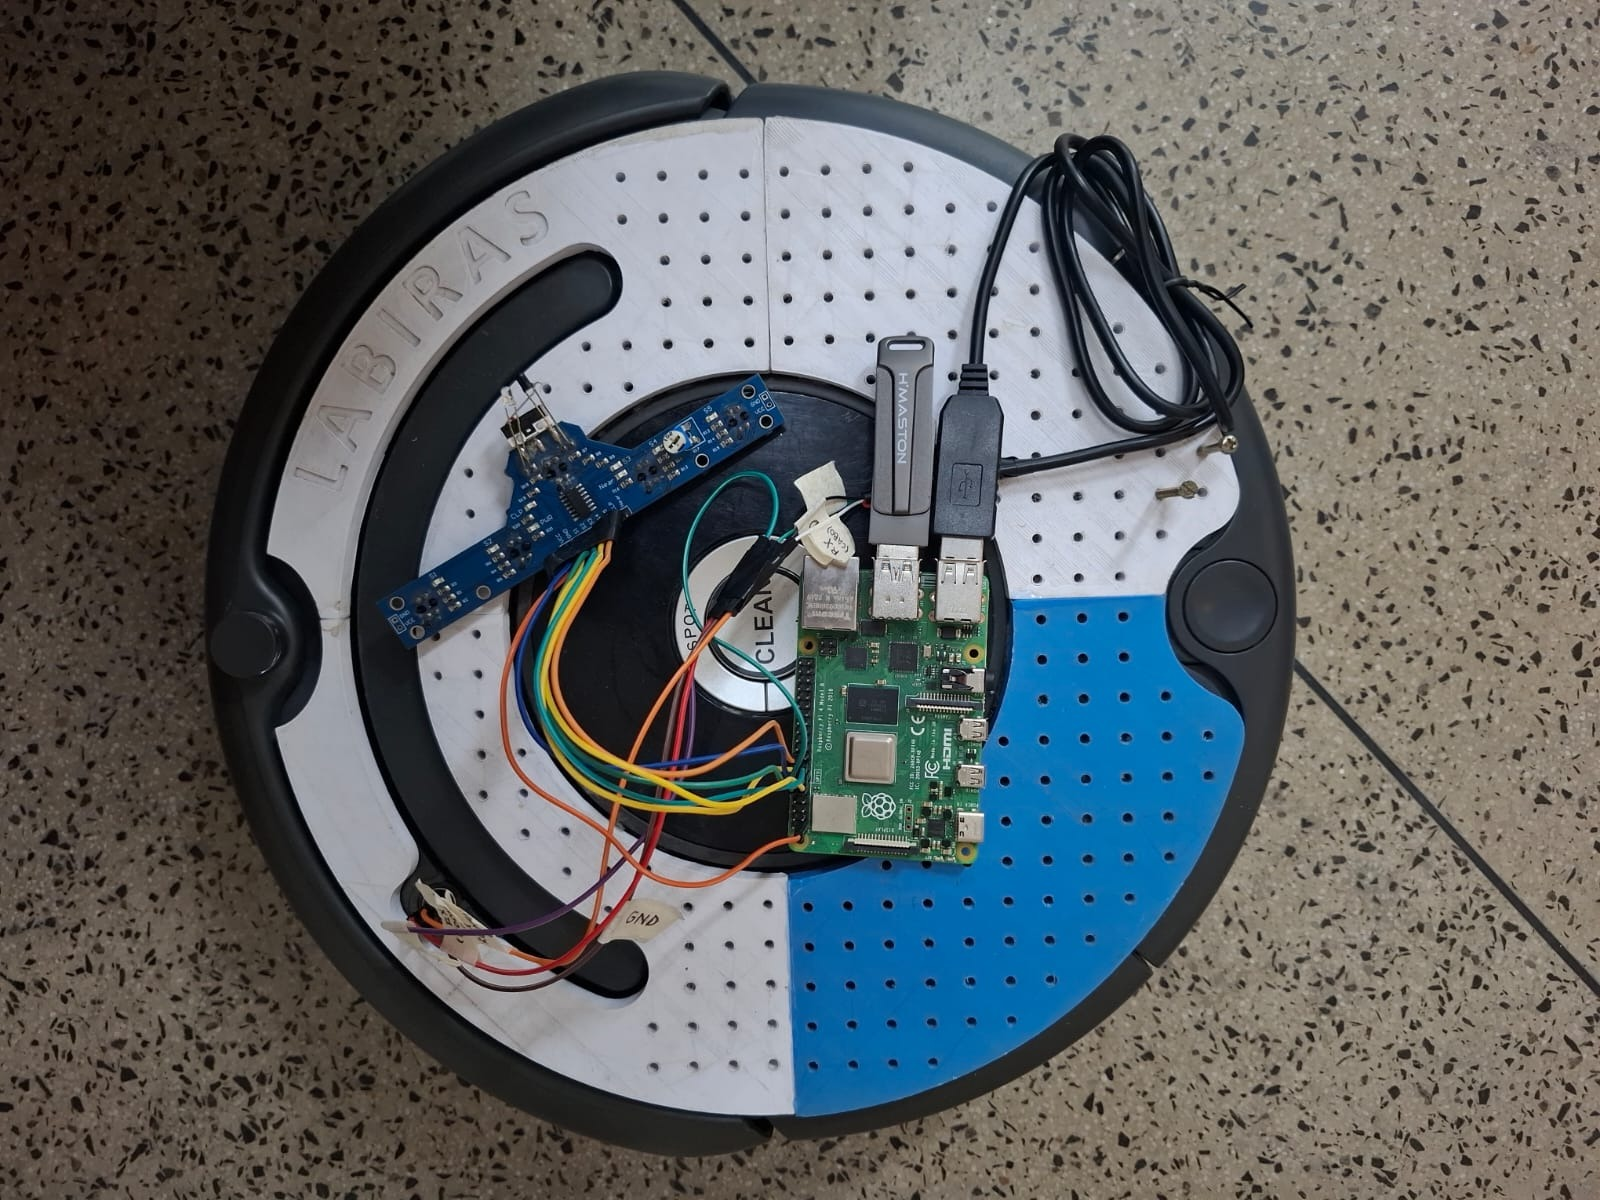
\includegraphics[width=0.5\textwidth]{imagens/componentes_hardware}
	\end{center}
	\legend{Fonte: Elaborado pelo autor.}
\end{figure}

\subsection{Hardware e Conectividade}

O iRobot Roomba 614 foi selecionado como base por sua robustez mecânica e facilidade de manutenção. Para o gerenciamento de energia do Raspberry Pi 4, optou-se pela utilização de uma \textit{powerbank} externa dedicada, com saída de 5V DC e capacidade de corrente suficiente para evitar o fenômeno de \textit{under-voltage}, garantindo a estabilidade operacional do ROS 2 e dos periféricos conectados.

A conectividade sensorial baseia-se em um módulo seguidor de linha BFD-1000, montado na parte frontal inferior do chassi. Este módulo é composto por 5 sensores infravermelhos integrados, onde cada sensor opera emitindo um feixe de luz infravermelha e medindo a reflexão retornada. Em superfícies escuras (como a linha preta), a reflexão é mínima, enquanto em superfícies claras (como a pista branca), a reflexão é alta. Essa variação analógica é digitalizada pelos pinos GPIO do Raspberry Pi através de um comparador de tensão integrado no módulo do sensor, permitindo uma leitura binária rápida (0 ou 1) que é processada a 20Hz.

\subsubsection{Interface de Sensores e Comunicação}
Utilizou-se o módulo BFD-1000 para obter as 5 leituras simultâneas de linha. A leitura é feita diretamente pelos pinos GPIO (BCM 17, 27, 22, 23, 24). O cálculo do erro de linha é feito por média ponderada: atribui-se pesos (-2, -1, 0, 1, 2) aos sensores, permitindo determinar o quão longe o robô está do centro da linha.

Para a comunicação com o Roomba, utilizou-se um \textbf{Cabo Conversor USB-Serial TTL}. Esta solução foi adotada após testes com conversores de nível lógico avulsos apresentarem ruídos excessivos. O cabo conecta-se à porta \textit{/dev/ttyUSB0} com baud rate de 115200. Para o controle do estado de \textit{Sleep}, o pino GPIO 18 (físico 12) é conectado ao pino \textit{Device Detect} (DD) do Roomba, enviando um pulso de ativação na inicialização.

\begin{figure}[H]
	\caption{\label{fig:montagem}Diagrama de conexões elétricas do sistema físico.}
	\begin{center}
	    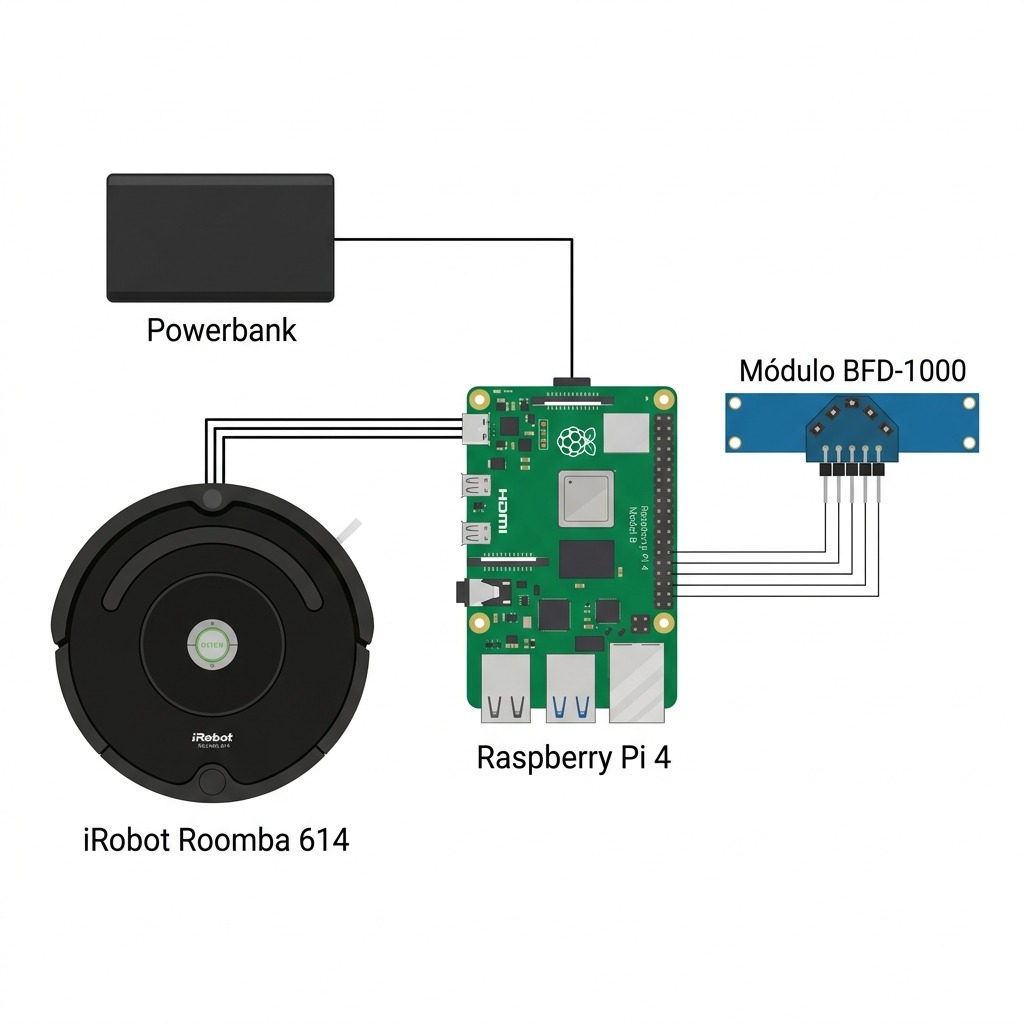
\includegraphics[width=0.6\textwidth]{imagens/diagrama_montagem_hardware}
	\end{center}
	\legend{Fonte: Elaborado pelo autor.}
\end{figure}

A modularidade é garantida pela divisão em pacotes orquestrados pelo framework \textit{ros2\_control} ou lógica direta de nós \cite{amadi2024ros2control}:
\begin{itemize}
    \item \textbf{\textit{roomba\_pi\_drivers}:} Inclui o \textit{motor\_driver.py} para tradução de velocidades (\textit{geometry\_msgs/Twist}) para o protocolo serial e o \textit{line\_sensor\_node.py} para leitura GPIO a 20Hz, publicando os dados em um tópico customizado;
    \item \textbf{\textit{roomba\_logic}:} Contém o \textit{pid\_controller\_node.py}, que implementa a Equação \ref{eq:pid_discreto}, e o \textit{mission\_control\_pi.py}, que atua como multiplexador de estados (\textit{StateMachine});
    \item \textbf{\textit{roomba\_bringup}:} Facilita a inicialização via \textit{launch files}, garantindo que os parâmetros de ganho PID sejam carregados dinamicamente no sistema.
\end{itemize}

\section{Resultados e Discussões}

O protótipo físico conseguiu realizar o seguimento de linha autônomo e contínuo. A malha de controle PID, rodando no Raspberry Pi 4, mostrou-se capaz de corrigir a trajetória em tempo real com baixa latência.

\subsection{Sintonia Experimental do PID}

A sintonia dos ganhos $K_p$, $K_i$ e $K_d$ seguiu um processo experimental iniciado no simulador e refinado no hardware físico. 
\begin{itemize}
    \item Primeiramente, elevou-se $K_p$ até que o robô apresentasse uma oscilação constante em torno da linha;
    \item Em seguida, introduziu-se o ganho $K_d$ para amortecer essa oscilação, permitindo que o robô enfrentasse curvas com maior suavidade;
    \item Por fim, o ganho $K_i$ foi ajustado para corrigir pequenos desvios sistemáticos acumulados durante longas retas ou irregularidades na pista.
\end{itemize}

A mitigação de ruído através do cabo USB-Serial foi um ponto crítico para o sucesso, permitindo uma comunicação estável sem perda de pacotes de comando mesmo em altas frequências de atualização. O sistema operou com uma taxa estável de 20 Hz, garantindo que o algoritmo PID físico executado no Raspberry Pi respondesse em tempo real. A abordagem de \textit{Edge Computing} mostrou-se fundamental para a estabilidade do controle físico e, simultaneamente, permitiu validar na simulação que a carga de processamento da visão computacional (OpenCV/ArUco) é compatível com os recursos da placa sem comprometer a latência da malha de controle.

A validação em simulação permitiu que o código de controle fosse portado para o físico com o mínimo de alterações na lógica, alterando-se apenas os ganhos de sintonia devido às diferenças de atrito e inércia do mundo real.

\begin{figure}[H]
	\caption{\label{fig:projeto_pronto}Robô em operação na pista de testes.}
	\begin{center}
	    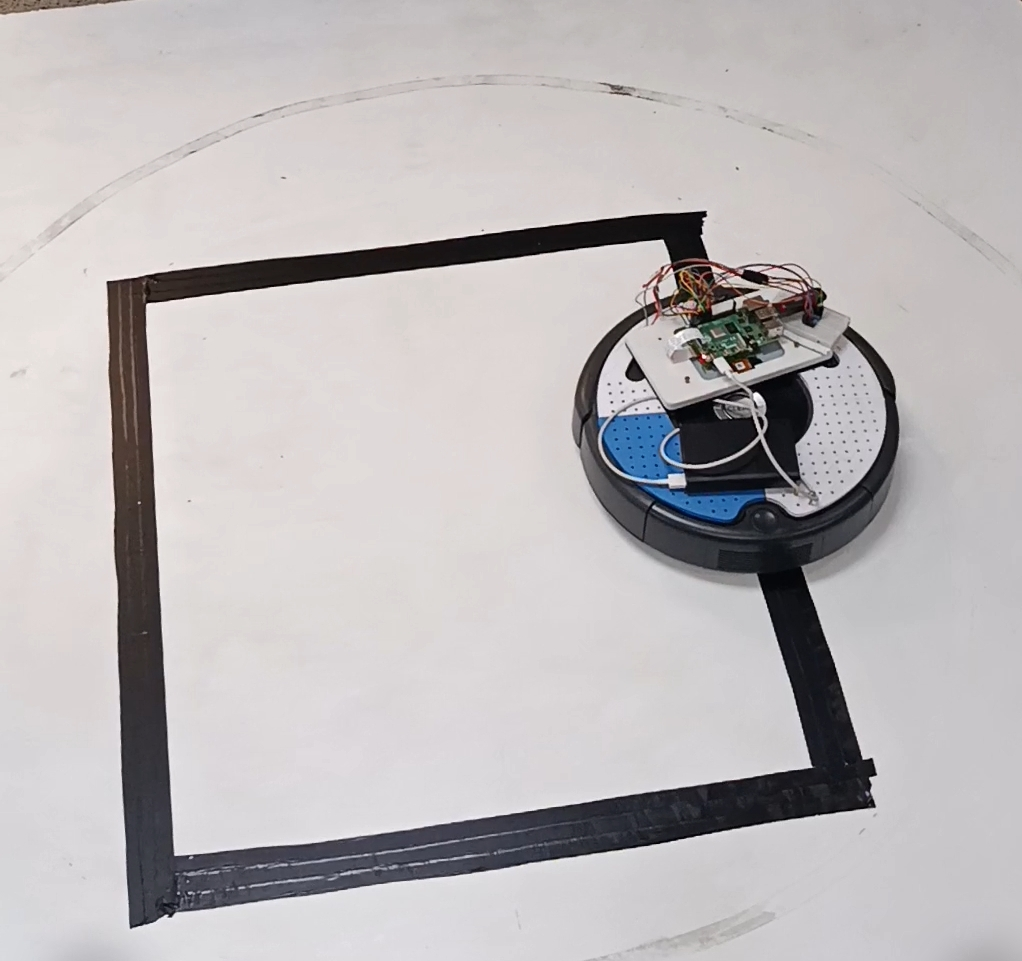
\includegraphics[width=0.5\textwidth]{imagens/roomba_funcionando_seguindo_linha}
	\end{center}
	\legend{Fonte: Elaborado pelo autor.}
\end{figure}
